%!TeX root=./tese.tex
% Figures are generated by predictors/figures_tex.py into
% predictors/results/figures/ and copied into figuras/pred/ (prefixed pred_).
% All numbers come from predictors/results/metrics/ (precision.py over the
% benchmark parquets produced by predictors/benchmark.py).
\chapter{Forecasting the Demand Signals with Time-Series Foundation Models}
\label{cap:predictors}

Chapter~\ref{cap:trace-eda} closed on a feasibility premise: the demand
signal most dangerous to reactive scaling --- the vision pool's image rate
--- is also the most persistent, retaining autocorrelation at exactly the
horizons provisioning needs. This chapter tests that premise directly. It
benchmarks three pretrained time-series foundation models used
\emph{zero-shot} --- Google's TimesFM-2.0-500M~\cite{Das2024TimesFM},
Amazon's Chronos-2 (120M)~\cite{Ansari2025Chronos2}, and Datadog's
Toto-2.0-2.5B~\cite{Khwaja2026Toto2} --- against three classical baselines
(naive persistence, exponential smoothing, and additive Holt--Winters
\cite{Hyndman2021fpp3}) on all four demand signals of the trace, at five
bin resolutions, under a single rolling-origin protocol. The questions are
the ones a predictive autoscaler poses: how accurate is the forecast at the
next step and across a 12-step horizon; whether conditioning on the other
signals (covariates) helps; and whether the models' native quantile bands
offer a better operating point than their point forecasts. Every number
and figure is reproducible from versioned scripts in the workspace
(\texttt{predictors/}), and the full forecast set --- 19.2 million
predicted values with nine quantiles each --- is archived in Parquet next
to the metric tables.

\section{Experimental protocol}
\label{sec:pred-protocol}

\paragraph{Series.} The materialized demand series of
Section~\ref{sec:eda-temporal} are used as-is: per-bin totals of requests,
images, context tokens, and generated tokens over the full seven days, at
resolutions of \SI{1}{\second}, \SI{15}{\second}, \SI{30}{\second},
\SI{45}{\second}, and \SI{1}{\minute} (604{,}800 down to 10{,}080 bins).

\paragraph{Rolling-origin grid.} A forecast \emph{origin} $o$ predicts
bins $[o, o{+}H)$ from the context window $[o{-}C, o)$, with horizon
$H{=}12$ steps at the native cadence of each series. Origins advance in
strides of $H$, so consecutive forecasts tile the timeline into a
continuous, non-overlapping prediction path --- the signal a scaler would
actually consume --- and every origin is a multiple of $H$, so all models
land on the same absolute bins wherever their context allows. The context
budget $C$ is each model's maximum context minus headroom for the forecast
tokens themselves, $(1\ \text{point} + 9\ \text{quantiles}) \times H = 120$
steps: $C = 1928$ for TimesFM (cap 2048), $3976$ for Toto-2 (cap 4096),
and $8072$ for Chronos-2 (cap 8192). The baselines are given the TimesFM
budget (1928). Cross-model comparisons are restricted to the
\emph{common span} --- origins ${\geq}\,8076$, predictable by every model
--- leaving 167 origins per model at \SI{1}{\minute} up to 49{,}727 at
\SI{1}{\second}.

\paragraph{Models and modes.} Every model forecasts every signal from its
own history alone (\emph{univariate} mode). The two models with a genuine
covariate mechanism are additionally run in \emph{covariate} mode:
Chronos-2 forecasts each target with the other three series supplied as
past-only covariates, its native conditioning path; Toto-2 forecasts all
four signals jointly as one multivariate series, so its variate-axis
attention mixes the signals. TimesFM has no covariate interface ---
covariate-blindness is precisely the request-rate-only ablation
conventional autoscalers embody. The baselines are configured
conventionally: exponential smoothing with $\alpha{=}0.3$; Holt--Winters
($\alpha{=}0.3$, $\beta{=}0.1$, $\gamma{=}0.1$) with a seasonal period of
one hour of bins where two full cycles fit the context window
(\SI{15}{\minute} at the \SI{1}{\second} resolution). Point forecasts are
the median for Chronos-2 and Toto-2, the mean head for TimesFM, and the
model value for the baselines, whose quantile bands are Gaussian
prediction intervals. All forecasts are floored at zero (rates are
non-negative). The nine quantile levels $0.1, \ldots, 0.9$ are the
intersection of the three models' native heads.

\paragraph{Metrics.} Accuracy is reported as WAPE, $\sum_t |\hat y_t -
y_t| \,/ \sum_t y_t$ --- a scale-free error that remains defined on bins
where the signal is zero --- alongside MAE where absolute units aid
interpretation. Metrics are computed at the first step ($h{=}1$), per
horizon step, and pooled over the horizon (\emph{overall}), for the point
forecast and for each quantile treated as a candidate point forecast. The
full benchmark --- 19.2M forecast values across eight model/mode
configurations --- runs in about \SI{2.5}{\hour} wall-clock on one
RTX~5090 (the baselines take about a minute each on CPU; Chronos-2 and
Toto-2 dominate at roughly one hour and 80 minutes).

\section{Point-forecast accuracy}
\label{sec:pred-point}

Table~\ref{tab:pred-wape} reports overall point WAPE on the common span at
the two extreme resolutions; Figure~\ref{fig:pred-heatmap} extends the
picture to all twenty (resolution, signal) cells and
Figure~\ref{fig:pred-horizon} resolves it across the horizon. Four
findings.

\begin{table}[htb]
\centering
\caption{Overall point-forecast WAPE (\%) on the common evaluation span,
pooled over the 12-step horizon. Bold marks the best model per column.}
\label{tab:pred-wape}
\small
\begin{tabular}{lrrrrcrrrr}
\toprule
& \multicolumn{4}{c}{\SI{1}{\minute} bins} & & \multicolumn{4}{c}{\SI{1}{\second} bins} \\
\cmidrule{2-5} \cmidrule{7-10}
Model & req & img & ctx & gen & & req & img & ctx & gen \\
\midrule
naive           & 42.3 & 67.8 & 55.4 & 51.0 & & 82.0 & 156.9 & 124.6 & 119.9 \\
EWMA            & 35.2 & 54.2 & 44.7 & 41.2 & & 68.1 & 146.1 & 106.0 & 100.0 \\
Holt--Winters   & 43.8 & 69.4 & 56.4 & 53.5 & & 93.9 & 217.0 & 151.5 & 143.7 \\
TimesFM         & 33.4 & 53.4 & \textbf{43.2} & 37.8 & & 66.3 & 120.5 & 95.8 & 89.5 \\
Chronos-2       & \textbf{33.4} & 53.1 & 43.4 & 38.0 & & 64.8 & 99.6 & 87.4 & 83.0 \\
Chronos-2 (cov) & 33.6 & \textbf{52.9} & 43.4 & 38.1 & & 64.8 & 99.3 & 87.0 & 82.3 \\
Toto-2          & 33.5 & 53.0 & 43.3 & 37.7 & & 63.0 & \textbf{98.8} & 86.2 & 82.1 \\
Toto-2 (cov)    & 33.6 & 53.1 & 43.3 & \textbf{37.4} & & \textbf{62.9} & 98.8 & \textbf{86.0} & \textbf{81.6} \\
\bottomrule
\end{tabular}
\end{table}

\begin{figure}[htb]
\centering
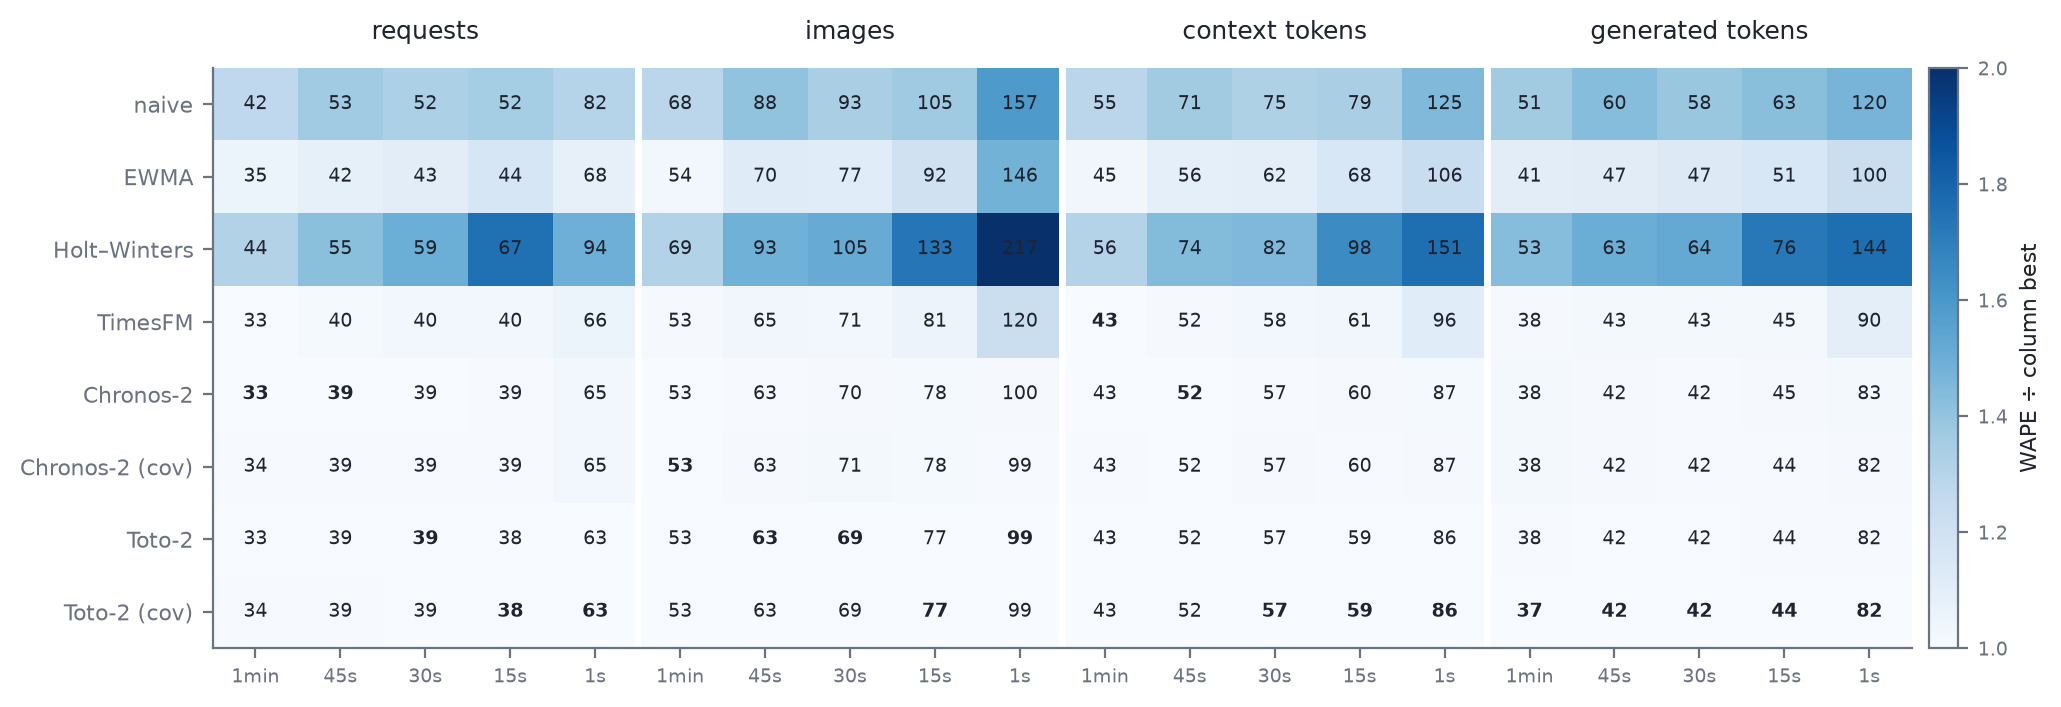
\includegraphics[width=\linewidth]{figuras/pred/pred_wape_heatmap.png}
\caption{Overall point WAPE (\%, annotated) for every model and every
(signal, resolution) cell on the common span; shading is each cell's WAPE
relative to the best model in its column, bold marks the column best. The
foundation-model rows are uniformly near-white --- within a few percent of
the per-cell optimum everywhere --- while the baseline rows darken as bins
shrink. Toto-2 with covariates carries most column wins at \SI{15}{\second}
and \SI{1}{\second}; Chronos-2 and TimesFM take the coarse-bin columns.
Holt--Winters is the worst model in every column --- worse than naive
persistence --- because extrapolating a fitted trend across a 12-step
horizon is precisely wrong for bursty, mean-reverting rates.}
\label{fig:pred-heatmap}
\end{figure}

\begin{figure}[htb]
\centering
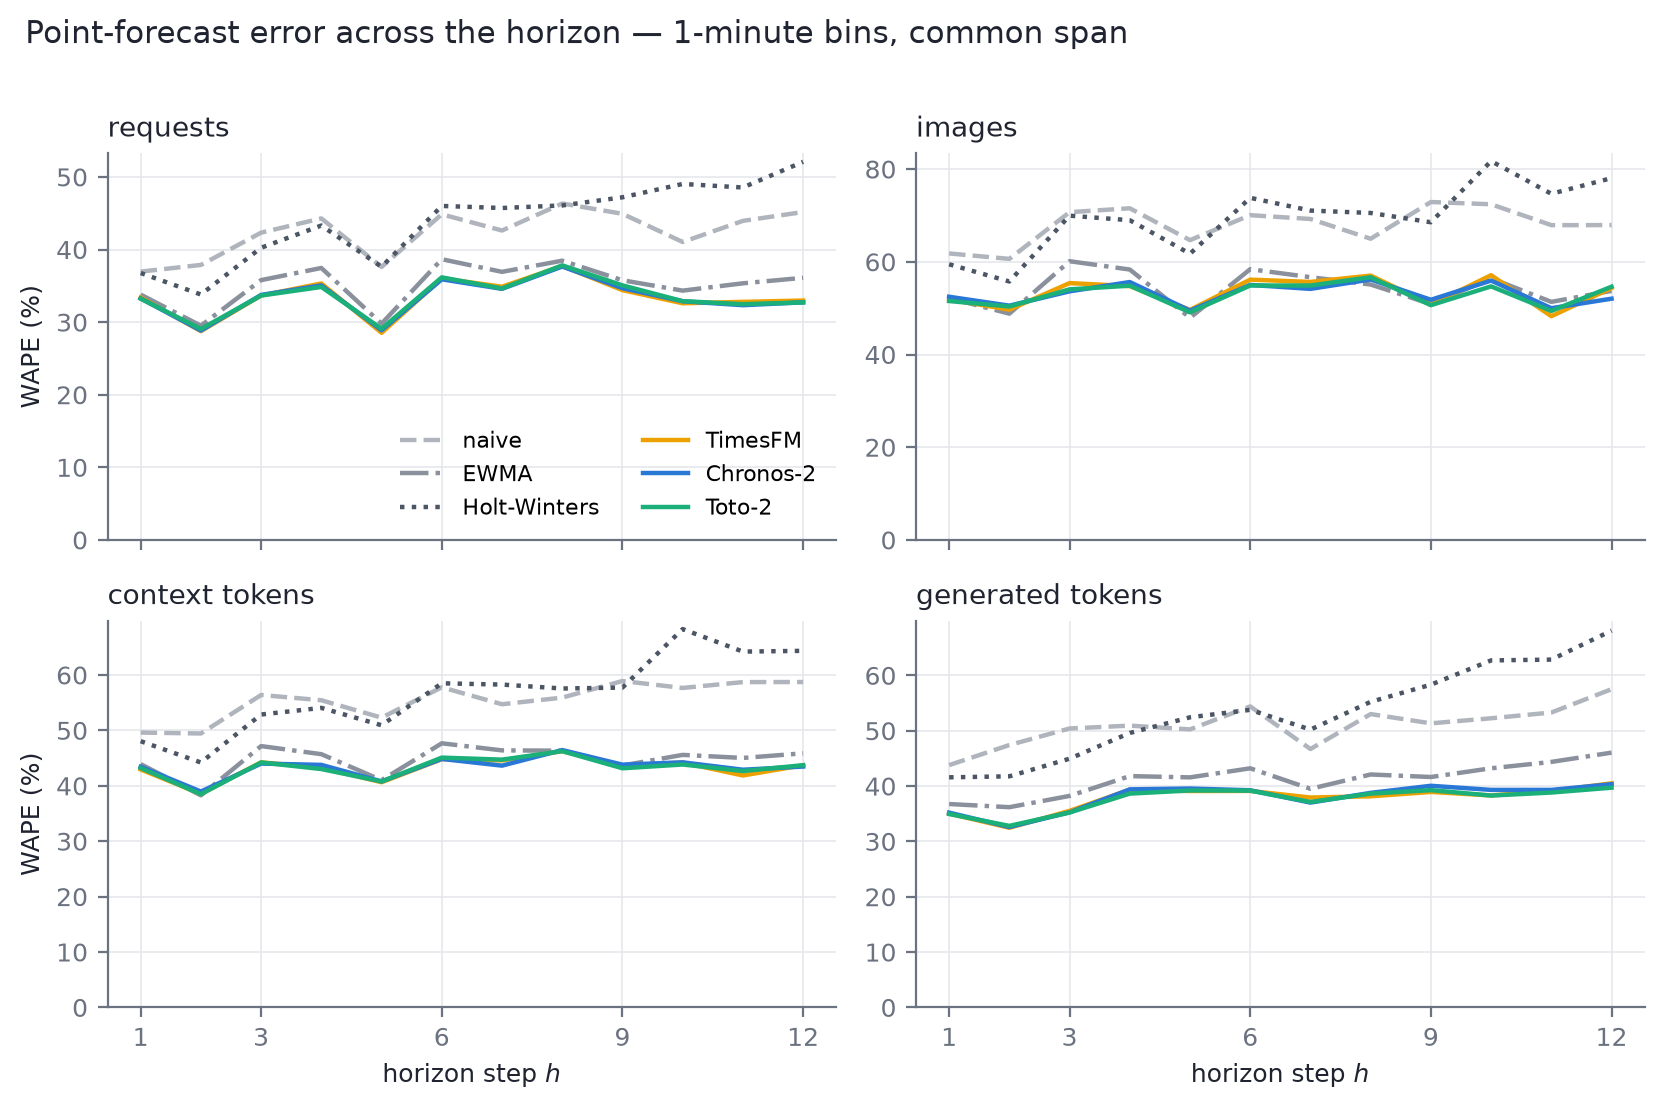
\includegraphics[width=\linewidth]{figuras/pred/pred_horizon_wape.png}
\caption{Point WAPE per horizon step at \SI{1}{\minute} (common span, 167
origins; the shared bin-to-bin zig-zag reflects which windows the common
span contains, not model noise). The three foundation models are nearly
indistinguishable and their error grows only a few points from $h{=}1$ to
$h{=}12$ --- the persistence found in Chapter~\ref{cap:trace-eda} is real
forecast capital. The gray baselines sit strictly above, and Holt--Winters
(dotted) degrades the fastest with $h$.}
\label{fig:pred-horizon}
\end{figure}

First, \textbf{the foundation models beat every baseline in all twenty
cells}, zero-shot, with no per-series tuning. The margin over the best
baseline (EWMA) is modest at \SI{1}{\minute} (e.g.\ images: 52.9\% vs.\
54.2\% WAPE) and widens dramatically as bins shrink: at \SI{1}{\second}
the best model forecasts images at 98.8\% WAPE against 146.1\% for EWMA
and 156.9\% for naive --- a one-third reduction exactly where reactive
signals are noisiest.

Second, \textbf{which model wins is resolution-dependent}. Toto-2
(usually with covariates) takes 15 of the 20 cells, all of them at
\SI{30}{\second} and finer; Chronos-2 leads the coarse-bin request and
image columns and TimesFM the \SI{1}{\minute} context column. The spreads
among the three are small (typically under 2 WAPE points), so model choice
matters far less than the choice to use a foundation model at all.

Third, \textbf{degradation across the horizon is mild}
(Figure~\ref{fig:pred-horizon}): for images at \SI{1}{\minute} the
foundation models move from ${\approx}52\%$ WAPE at $h{=}1$ to
${\approx}53\text{--}54\%$ at $h{=}12$, while naive drifts from 61.8\% to
67.9\% and Holt--Winters diverges. Twelve minutes of lead time is
essentially free once the model has the signal's long memory --- the
operational budget identified by the burst-onset analysis
(Section~\ref{sec:eda-vision}) is covered.

Fourth, the \textbf{absolute} error levels calibrate expectations: even
the best model carries ${\approx}53\%$ WAPE on 1-minute image bins and
${\approx}99\%$ on 1-second bins. The sub-minute floor is the white
shot-noise regime of Section~\ref{sec:eda-predictability} --- individual
$k^2$-image arrivals are not predictable, only their envelope is. In MAE
terms the best 1-minute forecasts miss by ${\approx}1{,}302$ images
(21.7 images/s against a common-span mean of ${\approx}41$ images/s ---
this evaluation span contains the week's largest burst), 35.6 requests,
166.6k context tokens, and 8.1k generated tokens per bin.

\section{Do covariates help?}
\label{sec:pred-covariates}

Table~\ref{tab:pred-cov} isolates the covariate effect: the mean relative
change in overall point MAE from univariate to covariate mode, per
resolution. The effect is marginal in both directions --- within
$\pm0.4\%$ everywhere --- but its structure is consistent: covariates
\emph{help} at \SI{15}{\second} and \SI{1}{\second} (both models,
strongest for Chronos-2 at $-0.39\%$) and are neutral-to-harmful at
coarser bins. This is the forecasting-side image of the decoupling result
of Section~\ref{sec:eda-vision}: the request-rate covariate explains only
$R^2{=}0.12$ of the image signal, so there is little cross-signal
information for the mechanism to exploit at horizons where each signal's
own history already carries its envelope; what remains surfaces only in
the shot-noise regime, where any extra conditioning signal has value.
The practical reading for a scaler is that per-pool forecasts can be run
univariate --- simpler and cheaper --- unless the system operates on
sub-15-second decision windows.

\begin{table}[htb]
\centering
\caption{Covariate effect: mean over the four signals of the relative
change in overall point MAE, covariate vs.\ univariate mode (common span;
negative = covariates help).}
\label{tab:pred-cov}
\begin{tabular}{lrrrrr}
\toprule
Model & \SI{1}{\minute} & \SI{45}{\second} & \SI{30}{\second} & \SI{15}{\second} & \SI{1}{\second} \\
\midrule
Chronos-2 & $+0.16\%$ & $+0.30\%$ & $+0.34\%$ & $-0.15\%$ & $-0.39\%$ \\
Toto-2    & $-0.04\%$ & $+0.08\%$ & $-0.02\%$ & $-0.25\%$ & $-0.24\%$ \\
\bottomrule
\end{tabular}
\end{table}

\section{Is any percentile a better operating point?}
\label{sec:pred-quantiles}

Each forecast carries nine quantiles, and a scaler need not consume the
point path --- it could provision against p60, or p40, or whatever level
tracks the signal best. Treating every quantile as a candidate point
forecast answers whether that is worth doing. Across the 160 (model,
mode, resolution, signal) cells, some quantile beats the point forecast
in 51 --- but the wins concentrate entirely in the models whose point
forecast is \emph{not} the median: TimesFM's mean head is beaten in 18 of
its 20 cells (median improvement $-1.7\%$, always by a below-median
quantile, modally p40), and the Gaussian-band baselines account for 31
more (up to $-45\%$ for Holt--Winters on 1-second images, where a p10
path simply undoes the model's burst overshoot). For Chronos-2 and
Toto-2, whose point \emph{is} the median, quantiles improve essentially
nothing (2 of 80 cells, ${\approx}0\%$). The pattern is what
right-skewed, bursty rates predict: the conditional median already sits
below the mean, so mean-like forecasts systematically overshoot after
spikes and a slightly pessimistic quantile corrects them. The operational
conclusion: with a median-point foundation model, the point path is
already the best single operating line, and the quantile band's role is
headroom sizing rather than point correction.

\section{The forecast as a scaling signal}
\label{sec:pred-signal}

Figure~\ref{fig:pred-band} renders the benchmark's output the way an
autoscaler would consume it, over the largest image burst of the week
(peak \num{370}~images/s on 2024-10-21, the episode of
Figure~\ref{fig:eda-sevenday}). Three properties matter operationally.
The point path tracks the burst \emph{plateau} --- the provisioning
envelope --- rather than chasing individual 1-minute spikes, which is the
desired behavior given the shot-noise floor. The p10--p90 band covers
nearly all observed excursions, giving a defensible headroom rule
(provision at p90 during regime uncertainty). And at the burst's collapse
the stitched path lags by up to one horizon (12 minutes), the price of
forecasting in $H$-step tiles; a scaler holding capacity 12 minutes too
long is a far cheaper failure than one arriving 6 minutes late to a
median-onset burst (Section~\ref{sec:eda-vision}).

\begin{figure}[htb]
\centering
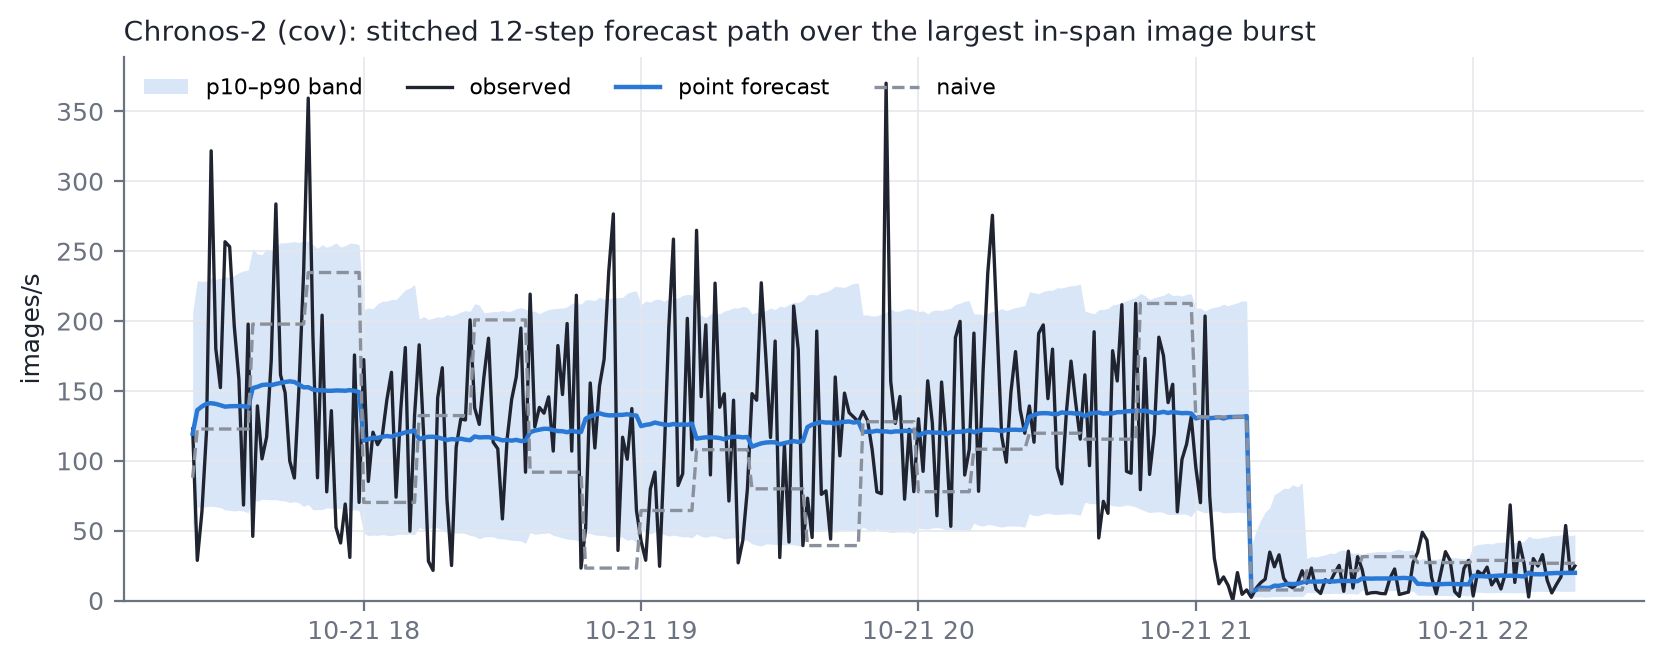
\includegraphics[width=\linewidth]{figuras/pred/pred_forecast_band.png}
\caption{Chronos-2 (covariate mode) over the week's largest image burst at
\SI{1}{\minute} resolution: observed signal (ink), stitched 12-step point
path (blue), p10--p90 band (shaded), and the naive path (dashed gray). The
forecast rides the burst plateau at ${\approx}120$--$150$ images/s while
individual bins spike to \num{370}~images/s inside the band, and it
releases the regime with at most a 12-minute (one-horizon) lag at the
collapse around 21:00.}
\label{fig:pred-band}
\end{figure}

\section{Limitations}
\label{sec:pred-limitations}

The benchmark inherits the trace's arrival-side construction: all signals
are offered-work rates stamped at arrival, so decode-side forecasts
predict offered load, not instantaneous decode occupancy. All models run
zero-shot; fine-tuning on the trace's first days could shift both the
absolute levels and the model ranking. The quantile analysis treats each
level as a candidate point path and does not assess calibration (coverage
of the nominal levels), which is the natural next question for
headroom-based provisioning. Chronos-2 occasionally emits locally crossed
quantiles (its head does not enforce monotonicity); values are recorded
raw. Finally, results derive from one seven-day trace of one production
cluster, with its by-construction 50/50 modality split.

\section{Summary}

Zero-shot time-series foundation models forecast all four demand signals
of the trace better than tuned classical baselines in every cell of a
$5{\times}4$ resolution--signal grid, with the largest margins (one-third
lower WAPE) at sub-minute bins, and their accuracy decays only marginally
across a 12-step horizon --- confirming that the persistence identified in
Chapter~\ref{cap:trace-eda} is exploitable in practice, at provisioning
lead times that cover the median burst onset. Cross-signal covariates are
nearly irrelevant at provisioning cadences --- the forecasting-side echo
of the pools' decoupling --- and for median-point models no fixed quantile
improves on the point path, leaving the band as headroom rather than
correction. The strongest model at fine resolutions (Toto-2 with joint
multivariate attention) and at coarse resolutions (Chronos-2) differ by
margins small enough that engineering considerations --- model size,
latency, covariate interface --- can drive the choice. These forecasts,
tiled contiguously at the serving cadence, are exactly the input the
predictive autoscaling experiments of the following chapters consume.
